\documentclass[tikz, convert={convertexe=magick}, png]{standalone}

\usepackage{yquant, braket}
\yquantset{register/default name=$\ket{\reg_{\idx}}$}

\begin{document}
   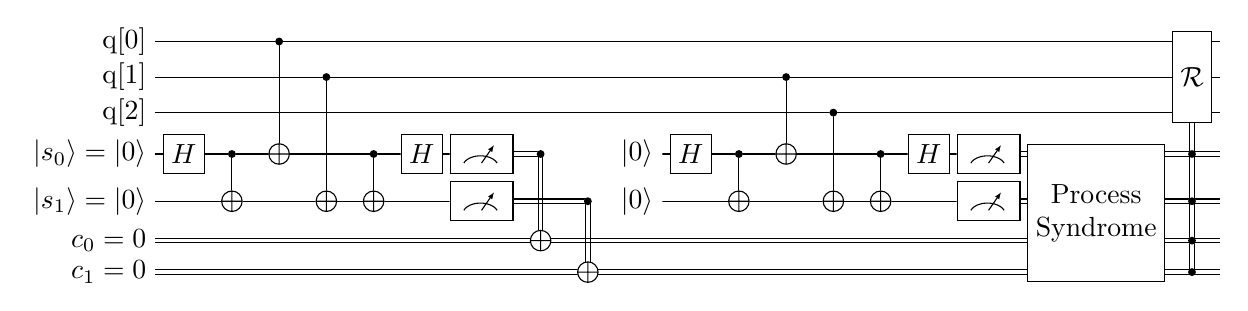
\begin{tikzpicture}
      \begin{yquant}
         qubit q[3];
         qubit {$\ket{s_{\idx}} = \ket0$} s[2];
         cbit {$c_{\idx} = 0$} c[2];
         
         h s[0];
         cnot s[1] | s[0];
         cnot s[0] | q[0];
         cnot s[1] | q[1];
         cnot s[1] | s[0];
         h s[0];
         measure s;
         cnot c[0] | s[0];
         cnot c[1] | s[1];
         discard s;
         
         init {$\ket0$} s;
         h s[0];
         cnot s[1] | s[0];
         cnot s[0] | q[1];
         cnot s[1] | q[2];
         cnot s[1] | s[0];
         h s[0];
         measure s;
         
         box {Process\\Syndrome} (s, c);
         box {$\mathcal R$} (q) | s, c;
      \end{yquant}
   \end{tikzpicture}
\end{document}